\documentclass[addpoints]{exam}
\usepackage{amsmath,amsthm,amssymb,url}
\usepackage{cancel}
\usepackage{algorithm}
\usepackage{algorithmic}
\usepackage{graphicx}
\usepackage{float}
\usepackage{upgreek}
\usepackage{bm}
\usepackage{units}
\usepackage[pdftex]{hyperref}
\usepackage{tikz}
\usepackage{subcaption}
\usetikzlibrary{shapes,snakes, patterns}

\def\checkmark{\hspace{.5em}\tikz\fill[scale=0.4](0,.35) -- (.25,0) -- (1,.7) -- (.25,.15) -- cycle;} 
\DeclareMathOperator*{\pprime}{\prime \prime}
\renewcommand{\algorithmicrequire}{\textbf{Input:}}
\renewcommand{\algorithmicensure}{\textbf{Output:}}
\newcommand{\BigO}[1]{\mathcal{O}\left( #1\right)}
\newcommand{\D}[1]{\left. #1 \right|_{i}^{n}}
\newcommand{\C}[1]{\cancel{ #1}}
\newcommand{\DC}[1]{\C{\D{ #1}}}
\newcommand{\Dx}{\Delta x}
\newcommand{\Dy}{\Delta y}
\newcommand{\Dt}{\Delta t}
\newcommand{\Dtp}{\Delta t^{\prime}}


\newtheorem{lemma}{Lemma}[section]
\newcommand{\var}{\text{Var}}
\title{ME EN 6720: Project 1}
\date{Due Date: April 7, 2016}
\author{Christopher Mertin}
\begin{document}
\maketitle
%\begin{center}
%\fbox{\fbox{\parbox{5.5in}{\centering
%This assignment has \numquestions\ questions, for a total of \numpoints\
%points.
%Unless otherwise specified, complete and reasoned arguments will be
%expected for all answers. 
%}}}
%\end{center}

\qformat{Question \thequestion: \thequestiontitle\dotfill}
\pointname{}
\bonuspointname{}
\pointformat{[\bfseries\thepoints]}

\printanswers



\begin{questions}
\titledquestion{Project 1}
This project will consist of developing your own solver code for the 2D incompressible Navier-Stokes equations. Consider the lid driven cavity flow depicted below in the figure. The top of the lid moves with a constant velocity $U$ in the $x$ direction and the cavity is square and each side of the cavity has a lenght $w$. The fluid in the cavity has kinematic viscosity $\nu$. Using a primitive variables formulation and the projection method, follow the algorithm on page 170 of Ferziger and Peri\'{c} (2002) to solve for the 2D flow field in the caivity.

{\bf Deliverables:}
\begin{itemize}
\item A description of your methodology including: The general method (i.e. pressure projection), your discretization schemes and grid layout, your chosen Poisson equation methodology, and your time advancement method.
\item Run at least two Reynolds numbers $R_{e} = Uw/\nu$ chosen to demonstrate ``high'' and ``low'' $R_{e}$ behavior (hint $R_{e} = 1,000$ should be ``high''). For each $R_{e}$, submit plots of the following during the initial flow development phase {\bf and} at steady-state:
\begin{itemize}
\item The velocity vectors in the cavity as a function of $x$ and $y$
\item The stream function in the cavity as a function of $x$ and $y$
\item The vorticity in the cavity as a function of $x$ and $y$
\end{itemize}
Note: It is acceptable to combine more than one (but not all three) of these plots together. For example, velocity vectors over vorticity. You should also include a short description of the differences in the dynamiocs of the two different simulations at their early development stage and stead-state stage.
\item Evidence of grid convergence for the high-$R_{e}$ case. Include a discussion justifying your criteria and the outcome of your tests.
\item Your code
\end{itemize}

\begin{figure}[H]
\centering
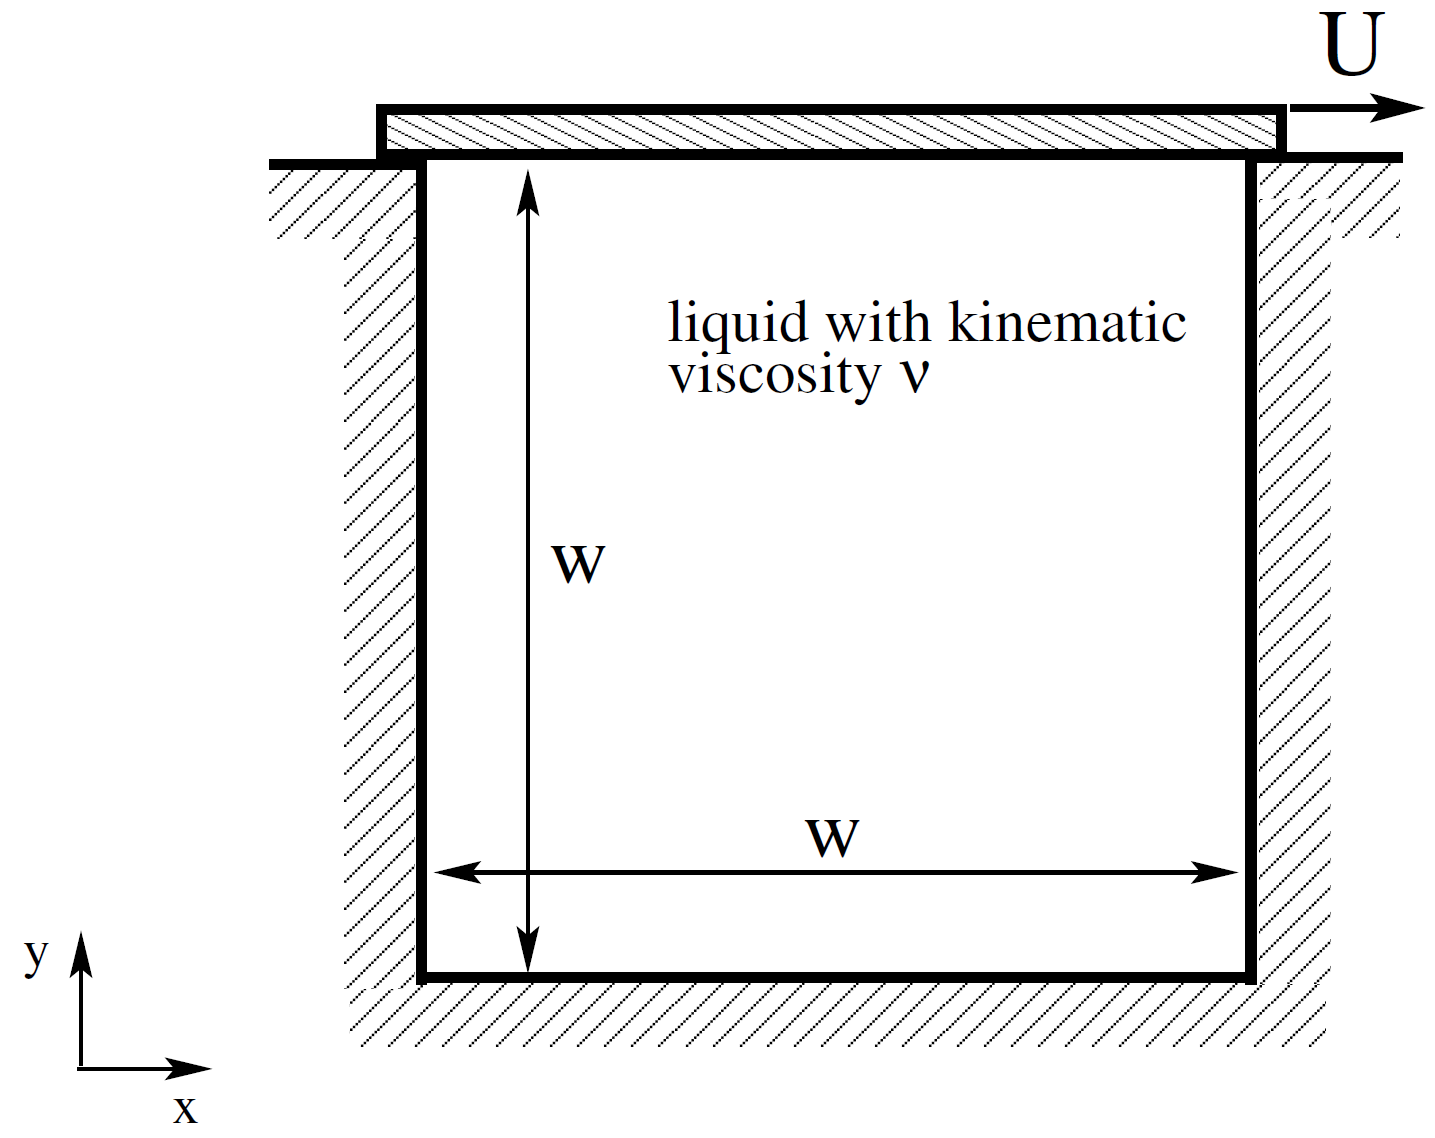
\includegraphics[width = .4\textwidth]{fig1.png}
\caption{Description of the system}
\end{figure}

\begin{solution}
The Navier-Stokes Equations need to satisfy the constraints of {\em Conservation of Mass} and {\em Conservation of Momentum}, where the equations are derived below.

{\bf \large Conservation of Mass}
To solve the system while conserving mass, the grid that was used was the staggered grid which can be seen in Figure~\ref{fig:stagg_1}. To conserve mass in the element, the following needs to be satisfied

\begin{align}
\oint_{s}\mathbf{u}\cdot \hat{n} \text{ d}s = 0
\end{align}

which simply states that the flow of the velocity in each component of the system. If we integrate over this boundary, and with $h = \Delta x = \Delta y$, we get

\begin{align}
hu_{i+\frac{1}{2},j}^{n+1} - hu_{i-\frac{1}{2},j}^{n+1} + hv_{i,j+\frac{1}{2}}^{n+1} - hv_{i,j-\frac{1}{2}}^{n+1} = 0
\intertext{where, if we divide by $h$ gives us}
u_{i+\frac{1}{2},j}^{n+1} - u_{i-\frac{1}{2},j}^{n+1} + v_{i,j+\frac{1}{2}}^{n+1} - v_{i,j-\frac{1}{2}}^{n+1} = 0
\end{align}

\begin{figure}[H]
\centering
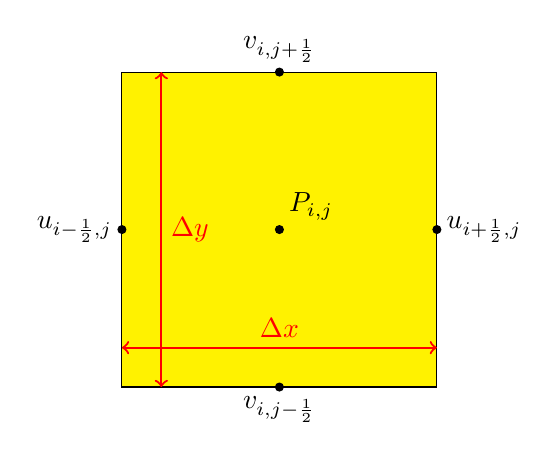
\begin{tikzpicture}
\draw [fill=yellow] (0, 0) rectangle (4,4);
\draw[fill] (0,2) circle[radius=0.05];
\draw[fill] (2,2) circle[radius=0.05];
\draw[fill] (4,2) circle[radius=0.05];
\draw[fill] (2,0) circle[radius=0.05];
\draw[fill] (2,4) circle[radius=0.05];
\node [right] at (4,2) {$u_{i+\frac{1}{2},j}$};
\node [left] at (0,2) {$u_{i-\frac{1}{2},j}$};
\node [below] at (2,0) {$v_{i,j-\frac{1}{2}}$};
\node [above] at (2,4) {$v_{i,j+\frac{1}{2}}$};
\node [above right] at (2,2) {$P_{i,j}$};
\node [right, red] at (0.5,2) {$\Delta y$};
\node [above, red] at (2,0.5) {$\Delta x$};
\draw [thick, red, <->] (0.5,0) -- (0.5,4);
\draw [thick, red, <->] (0, 0.5) -- (4, 0.5);
\end{tikzpicture}
\caption{Staggered Grid: Single Cell}
\label{fig:stagg_1}
\end{figure}

\newpage
{\bf \large Conservation of Momentum: Advection Terms}

\begin{figure}[H]
\centering
\begin{minipage}{.4\textwidth}
\centering
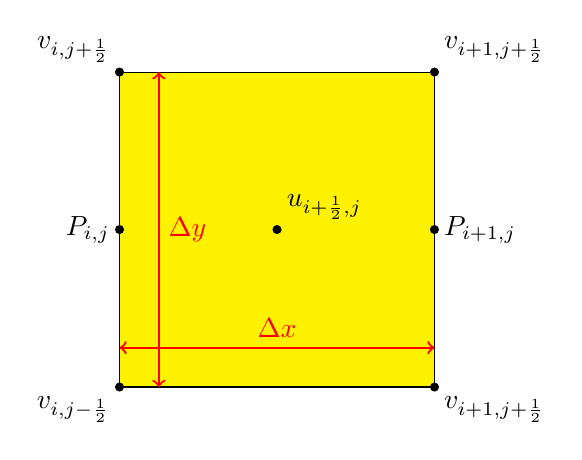
\begin{tikzpicture}
\draw [fill=yellow] (0, 0) rectangle (4,4);
\draw[fill] (0,2) circle[radius=0.05];
\draw[fill] (2,2) circle[radius=0.05];
\draw[fill] (4,2) circle[radius=0.05];
\draw[fill] (0,4) circle[radius=0.05];
\draw[fill] (4,4) circle[radius=0.05];
\draw[fill] (0,0) circle[radius=0.05];
\draw[fill] (4,0) circle[radius=0.05];
\node [right] at (4,2) {$P_{i+1,j}$};
\node [left] at (0,2) {$P_{i,j}$};
\node [above left] at (0,4) {$v_{i,j+\frac{1}{2}}$};
\node [above right] at (4,4) {$v_{i+1,j+\frac{1}{2}}$};
\node [below left] at (0,0) {$v_{i,j-\frac{1}{2}}$};
\node [below right] at (4,0) {$v_{i+1,j+\frac{1}{2}}$};
\node [above right] at (2,2) {$u_{i+\frac{1}{2},j}$};
\node [right, red] at (0.5,2) {$\Delta y$};
\node [above, red] at (2,0.5) {$\Delta x$};
\draw [thick, red, <->] (0.5,0) -- (0.5,4);
\draw [thick, red, <->] (0, 0.5) -- (4, 0.5);
\end{tikzpicture}
\captionof{figure}{Control Volume for $u$}
\label{fig:stagg_u}
\end{minipage}
\hspace{5em}
\begin{minipage}{.4\textwidth}
\centering
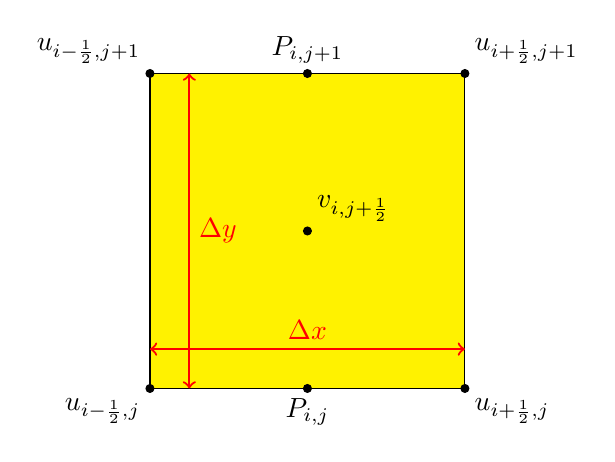
\begin{tikzpicture}
\draw [fill=yellow] (0, 0) rectangle (4,4);
\draw[fill] (2,0) circle[radius=0.05];
\draw[fill] (2,2) circle[radius=0.05];
\draw[fill] (2,4) circle[radius=0.05];
\draw[fill] (0,4) circle[radius=0.05];
\draw[fill] (4,4) circle[radius=0.05];
\draw[fill] (0,0) circle[radius=0.05];
\draw[fill] (4,0) circle[radius=0.05];
\node [above] at (2,4) {$P_{i,j+1}$};
\node [below] at (2,0) {$P_{i,j}$};
\node [above left] at (0,4) {$u_{i-\frac{1}{2},j+1}$};
\node [above right] at (4,4) {$u_{i+\frac{1}{2},j+1}$};
\node [below left] at (0,0) {$u_{i-\frac{1}{2},j}$};
\node [below right] at (4,0) {$u_{i+\frac{1}{2},j}$};
\node [above right] at (2,2) {$v_{i,j+\frac{1}{2}}$};
\node [right, red] at (0.5,2) {$\Delta y$};
\node [above, red] at (2,0.5) {$\Delta x$};
\draw [thick, red, <->] (0.5,0) -- (0.5,4);
\draw [thick, red, <->] (0, 0.5) -- (4, 0.5);
\end{tikzpicture}
\captionof{figure}{Control Volume for $v$}
\label{fig:stagg_v}
\end{minipage}
\end{figure}

For the momenum conservation, we can define the control volumes for $u$ and $v$ as seen in Figure~\ref{fig:stagg_u} and Figure~\ref{fig:stagg_v}. To find the momenum conservation, we need to define the cell averages. The elements of each cell are defined in Figure~\ref{fig:avg}.

\begin{figure}[H]
\centering
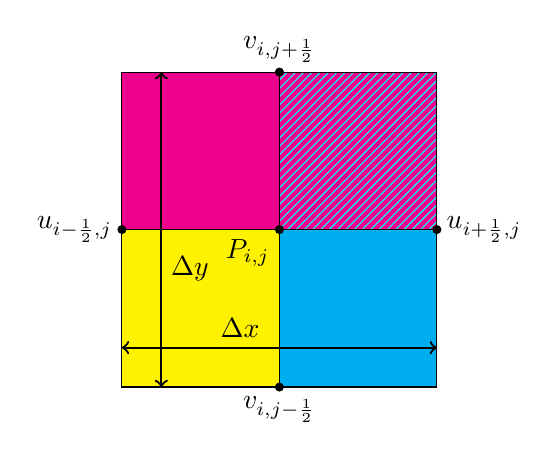
\begin{tikzpicture}
\draw [fill=yellow] (0, 0) rectangle (4,4);
\draw [fill=cyan] (2,0) rectangle(4,2);
\draw [fill=magenta] (0,2) rectangle(4,4);
\draw [pattern = north east lines, pattern color=cyan] (2,2) rectangle(4,4);
\draw[fill] (0,2) circle[radius=0.05];
\draw[fill] (2,2) circle[radius=0.05];
\draw[fill] (4,2) circle[radius=0.05];
\draw[fill] (2,0) circle[radius=0.05];
\draw[fill] (2,4) circle[radius=0.05];
\node [right] at (4,2) {$u_{i+\frac{1}{2},j}$};
\node [left] at (0,2) {$u_{i-\frac{1}{2},j}$};
\node [below] at (2,0) {$v_{i,j-\frac{1}{2}}$};
\node [above] at (2,4) {$v_{i,j+\frac{1}{2}}$};
\node [below left] at (2,2) {$P_{i,j}$};
\node [right, black] at (0.5,1.5) {$\Delta y$};
\node [above, black] at (1.5,0.5) {$\Delta x$};
\draw [thick, black, <->] (0.5,0) -- (0.5,4);
\draw [thick, black, <->] (0, 0.5) -- (4, 0.5);
\end{tikzpicture}
\caption{Contributions from each cell, magenta is from the $v$-cell, cyan is from $u$-cell, and yellow is the normal $P$ node, which composes the {\em enitre} domain, but the $v$ and $u$ cells were shown to be dominate to see the domain they cover.}
\label{fig:avg}
\end{figure}

The equations that define these averages are defined as

\begin{align}
u &= \frac{1}{V}\int_{V_{u}}u\ \text{d}V\\
v &= \frac{1}{V}\int_{V_{v}}v\ \text{d}V\\ 
P &= \frac{1}{V}\int_{V_{P}}p\ \text{d}V
\intertext{where we can define the {\em change of $x$-momentum} as from Figure~\ref{fig:stagg_u}}
\frac{\partial}{\partial t}&\int_{V}u\ \text{d}V
\intertext{where if we integrate over the control volume gives us}
\frac{\partial}{\partial t}\int_{V}u\ \text{d}V &\approx \frac{u_{i+\frac{1}{2},j}^{n+1} - u_{i+\frac{1}{2},j}^{n}}{\Delta t}h^{2}
\intertext{which can be done for the {\em change of $y$-momentum} as from Figure~\ref{fig:stagg_v}, giving}
\frac{\partial}{\partial t}\int_{V}v\ \text{d}V &\approx \frac{v_{i,j+\frac{1}{2}}^{n+1} - v_{i,j+\frac{1}{2}}^{n}}{\Delta t}h^{2}
\intertext{We also need to define the in/out flow of the $x$-momentum, which can be calculated as}
\oint_{S}u\mathbf{u}\cdot \hat{n}\ \text{d}S &\approx \left( \left(u^{2}\right)_{i+1,j}^{n} - \left(u^{2}\right)_{i,j}^{n} + (uv)^{n}_{i+\frac{1}{2},j+\frac{1}{2}} - (uv)^{n}_{i+\frac{1}{2},j-\frac{1}{2}}\right)h
\intertext{and for the $y$-momentum}
\oint_{S}v\mathbf{u}\cdot \hat{n}\ \text{d}S &\approx \left( (uv)_{i+\frac{1}{2},j+\frac{1}{2}}^{n} - (uv)_{i-\frac{1}{2},j+\frac{1}{2}}^{n} + \left(v^{2}\right)^{n}_{i,j+1} - \left(v^{2}\right)^{n}_{i,j}\right)h
\intertext{where}
\left(u^{2}\right)^{n}_{i+1,j} &= \left[ \frac{1}{2}\left(u_{i+\frac{3}{2},j}^{n} + u_{i+\frac{1}{2},j}^{n}\right)\right]^{2}\\
\left(u^{2}\right)^{n}_{i,j} &= \left[ \frac{1}{2}\left( u_{i+\frac{1}{2},j}^{n} + u_{i-\frac{1}{2},j}^{n} \right) \right]^{2}\\
\left(uv\right)^{n}_{i+\frac{1}{2},j+\frac{1}{2}} &= \left[\frac{1}{2}\left( u_{i+\frac{1}{2},j}^{n} + u_{i+\frac{1}{2},j+1}^{n}\right)\right]\left[\frac{1}{2}\left( v_{i,j+\frac{1}{2}}^{n}+v_{i+1,j+\frac{1}{2}}^{n}\right)\right]\\
\left( uv\right)^{n}_{i+\frac{1}{2},j-\frac{1}{2}} &= \left[ \frac{1}{2}\left( u_{i+\frac{1}{2},j}^{n} + u_{i+\frac{1}{2},j-1}\right)\right] \left[ \frac{1}{2}\left( v_{i,j-\frac{1}{2}}^{n} + v_{i+1,j-\frac{1}{2}}^{n}\right)\right]\\
\left(v^{2}\right)_{i,j+1}^{n} &= \left[\frac{1}{2} \left( v_{i,j+\frac{3}{2}}^{n} + v_{i,j+\frac{1}{2}}^{n}\right)\right]^{2}\\
\left(v^{2}\right)_{i,j}^{n} &= \left[ \frac{1}{2}\left(v_{i,j+\frac{1}{2}}^{n} + v_{i,j-\frac{1}{2}}^{n}\right)\right]^{2}\\
(uv)^{n}_{i+\frac{1}{2},j+\frac{1}{2}} &= \left[ \frac{1}{2}\left(u_{i+\frac{1}{2},j}^{n} + u_{i+\frac{1}{2},j+1}^{n}\right)\right]\left[\frac{1}{2}\left(v_{i,j+\frac{1}{2}}^{n} + v_{i+1,j+\frac{1}{2}}^{n}\right)\right]\\
(uv)^{n}_{i-\frac{1}{2},j+\frac{1}{2}} &= \left[ \frac{1}{2}\left( u_{i-\frac{1}{2}}^{n} + u_{i-\frac{1}{2},j+1}^{n}\right) \right] \left[ \frac{1}{2} \left(v_{i,j+\frac{1}{2}}^{n} + v_{i-1,j+\frac{1}{2}}^{n}\right)\right]
\end{align}

Where the above equations were derived from Figure~\ref{fig:stagg_u} and Figure~\ref{fig:stagg_v}.

\newpage
{\bf \large Conservation of Momentum: Pressure Terms}


From Figure~\ref{fig:stagg_u}, it's easy to see that the pressure in the $x$-direction is given by

\begin{align}
\frac{1}{\rho}\oint_{S}pn_{x}\ \text{d}S &\approx \frac{1}{\rho}\left(p_{i+1,j} - p_{i,j}\right)h
\intertext{and equally for the $y$-direction from Figure~\ref{fig:stagg_v}}
\frac{1}{\rho}\oint_{S}pn_{y}\ \text{d}S &\approx \frac{1}{\rho}\left(p_{i,j+1} - p_{i,j}\right)h
\end{align}

{\bf \large Conservation of Momentum: Viscous Terms}

\begin{figure}[H]
\centering
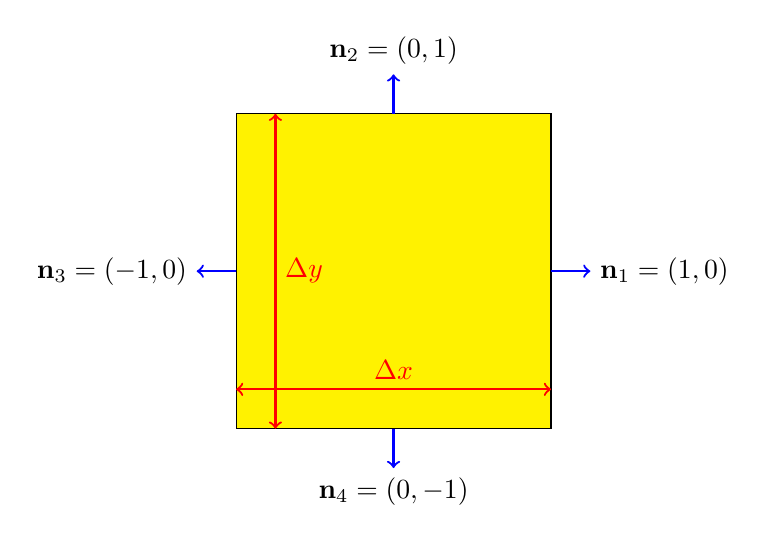
\begin{tikzpicture}
\draw [fill=yellow] (0, 0) rectangle (4,4);
\node [right, red] at (0.5,2) {$\Delta y$};
\node [above, red] at (2,0.5) {$\Delta x$};
\draw [thick, red, <->] (0.5,0) -- (0.5,4);
\draw [thick, red, <->] (0, 0.5) -- (4, 0.5);
\draw [thick, blue, ->] (4,2) -- (4.5,2);
\node [right] at (4.5,2) {$\mathbf{n}_{1}=(1,0)$};

\draw [thick, blue, ->] (2,4) -- (2,4.5);
\node [above] at (2,4.5) {$\mathbf{n}_{2}=(0,1)$};

\draw [thick, blue, ->] (0,2) -- (-0.5,2);
\node [left] at (-0.5,2) {$\mathbf{n}_{3}=(-1,0)$};

\draw [thick, blue, ->] (2,0) -- (2,-0.5);
\node [below] at (2,-0.5) {$\mathbf{n}_{4}=(0,-1)$};
\end{tikzpicture}
\caption{Viscous diffusion}
\label{fig:stagg_diffusion}
\end{figure}

where we can approximate the integral as

\begin{align}
\nu\oint_{S}\nabla u\cdot \hat{n}\ \text{d}S &= \nu\oint_{S}\left(\frac{\partial u}{\partial x}n_{x} + \frac{\partial u}{\partial y}n_{y}\right)\ \text{d}S\\
&\approx \nu\left[ \left.\frac{\partial u}{\partial x}\right|_{1}h + \left.\frac{\partial u}{\partial y}\right|_{2}h - \left.\frac{\partial u}{\partial x}\right|_{3}h - \left.\frac{\partial u}{\partial y}\right|_{4}h \right]\\
&\approx \nu\left[ \left.\frac{\partial u}{\partial x}\right|_{i+1,j}^{n} + \left.\frac{\partial u}{\partial y}\right|_{i,j}^{n} - \left.\frac{\partial u}{\partial x}\right|_{i+\frac{1}{2},j+\frac{1}{2}}^{n} - \left.\frac{\partial u}{\partial y}\right|_{i+\frac{1}{2},j-\frac{1}{2}}^{n} \right]h
\intertext{which if we discritize gives us the final result of}
\nu\oint_{S}\nabla u\cdot \hat{n}\ \text{d}S &\approx \nu\left(u_{i+\frac{3}{2},j}^{n} + u_{i-\frac{1}{2},j}^{n} + u_{i+\frac{1}{2},j+1}^{n} + u_{i+\frac{1}{2},j-1}^{n} - 4u_{i+\frac{1}{2},j}^{n}\right)
\intertext{and similiarly for the $y$-diffusion momentum gives}
\nu\oint_{S}\nabla v\cdot \hat{n}\ \text{d}S &\approx \nu\left( v_{i,j+\frac{3}{2}}^{n} + v_{i,j-\frac{1}{2}}^{n} + v_{i+1,j+\frac{1}{2}}^{n} + v_{i-1,j+\frac{1}{2}}^{n} - 4v_{i,j+\frac{1}{2}}^{n}\right)
\end{align}

{\bf \large Combining Conservation Equations}

By combining the above conservation equations gives

\begin{align}
\frac{\partial}{\partial t} \int_{V}u\ \text{d}V &= -\oint_{S}u\mathbf{u}\cdot \hat{n}\ \text{d}S + \nu\oint_{S}\nabla u\cdot \hat{n}\ \text{d}S - \frac{1}{\rho}\oint_{S} pn_{x}\ \text{d}S
\intertext{where we can set $P = \frac{p}{\rho}$, making it}
\frac{\partial}{\partial t} \int_{V}u\ \text{d}V &= -\oint_{S}u\mathbf{u}\cdot \hat{n}\ \text{d}S + \nu\oint_{S}\nabla u\cdot \hat{n}\ \text{d}S - \oint_{S} Pn_{x}\ \text{d}S
\end{align}

where we can discritize this with the above equations that were defined.

{\bf \large Description of Solution Technique}

The above momentum equations can be rewritten as a single vector equation

\begin{align}
\frac{\mathbf{u}_{i,j}^{n+1}-\mathbf{u}_{i,j}^{n}}{\Delta t} &= -\mathbf{A}_{i,j}^{n} - \nabla_{h}P_{i,j} + \mathbf{D}_{i,j}^{n}\label{eq:vel}
\intertext{with $\mathbf{A}$ being the advection term, and $\mathbf{D}$ being the diffusiveness term. The mass conservation equations can be written as a {\em constraint} for our velocity update which is}
\nabla_{h}\cdot \mathbf{u}_{i,j}^{n+1} &= 0\label{eq:vel_constraint}
\intertext{where Equation~\ref{eq:vel} can be used as the Evolution of the velocity. However, there is no explicit equation for the velocity, but can be solved in the following way. We can split Equation~\ref{eq:vel} into}
\frac{\mathbf{u}_{i,j}^{t}-\mathbf{u}_{i,j}^{n}}{\Delta t} &= -\mathbf{A}_{i,j}^{n} + \mathbf{D}_{i,j}^{n}\Rightarrow \mathbf{u}_{i,j}^{t} = \mathbf{u}_{i,j}^{n} + \Delta t \left(-\mathbf{A}_{i,j}^{n} + \mathbf{D}_{i,j}^{n}\right)\\
\intertext{and}
\frac{\mathbf{u}_{i,j}^{n+1} - \mathbf{u}_{i,j}^{t}}{\Delta t} &= -\nabla_{h}P_{i,j} \Rightarrow \mathbf{u}_{i,j}^{n+1} = \mathbf{u}_{i,j}^{t} - \Delta t \nabla_{h}P_{i,j}\label{eq:vel_new}
\intertext{where a temporary velocity $\mathbf{u}^{t}$ was introduced to split the equation. To derive the equation for Pressure, we can take the divergence of \ref{eq:vel_new}, and with the constraint given in Equation~\ref{eq:vel_constraint} gives}
\cancel{\nabla_{h}\cdot \mathbf{u}_{i,j}^{n+1}} &= \nabla_{h}\cdot \mathbf{u}_{i,j}^{t} - \Delta t \nabla_{h}\cdot \nabla_{h}P_{i,j}\\
\Rightarrow \nabla_{h}^{2}P_{i,j} &= \frac{1}{\Delta t}\nabla_{h}\cdot \mathbf{u}_{i,j}^{t}
\end{align}

which now gives us all the equations that we need to solve the system of equations. To solve the system, we take the following steps:

\newpage
\begin{enumerate}
\item Impose Boundary Conditions
\item Find a temporary velocity using the advection and the diffusion terms only
\begin{align}
\mathbf{u}_{i,j}^{t} &= \mathbf{u}_{i,j}^{n} + \Delta t \left( - \mathbf{A}_{i,j}^{n} + \mathbf{D}_{i,j}^{n}\right)
\end{align}
\item Find the pressure needed to make the velocity field incompressible
\begin{align}
\nabla^{2}_{h}P^{n+1}_{i,j} &= \frac{1}{\Delta t}\nabla_{h}\cdot \mathbf{u}_{i,j}^{t}
\end{align}
\item Correct the velocity by adding the pressure gradient
\begin{align}
\mathbf{u}_{i,j}^{n+1} &= \mathbf{u}_{i,j}^{t} - \Delta t \nabla_{h}P_{i,j}\label{eq:vel_corr}
\end{align}
\item Return to 1 if $\left|\left| P^{n} - P^{n-1}\right|\right|_{2} > \text{tolerance}$
\end{enumerate}

{\bf \large Staggered Grid}

A full implementation of the staggered grid can be seen in Figure~\ref{fig:stagg_grid}. The array dimensions are as follows:

\begin{align}
&P(1\ldots N_{x}+1,1\ldots N_{y}+1)\\
&u(1\ldots N_{x},1\ldots N_{y}+1)\\
&v(1\ldots N_{x}+1,1\ldots N_{y})
\end{align}

\begin{figure}[H]
\centering
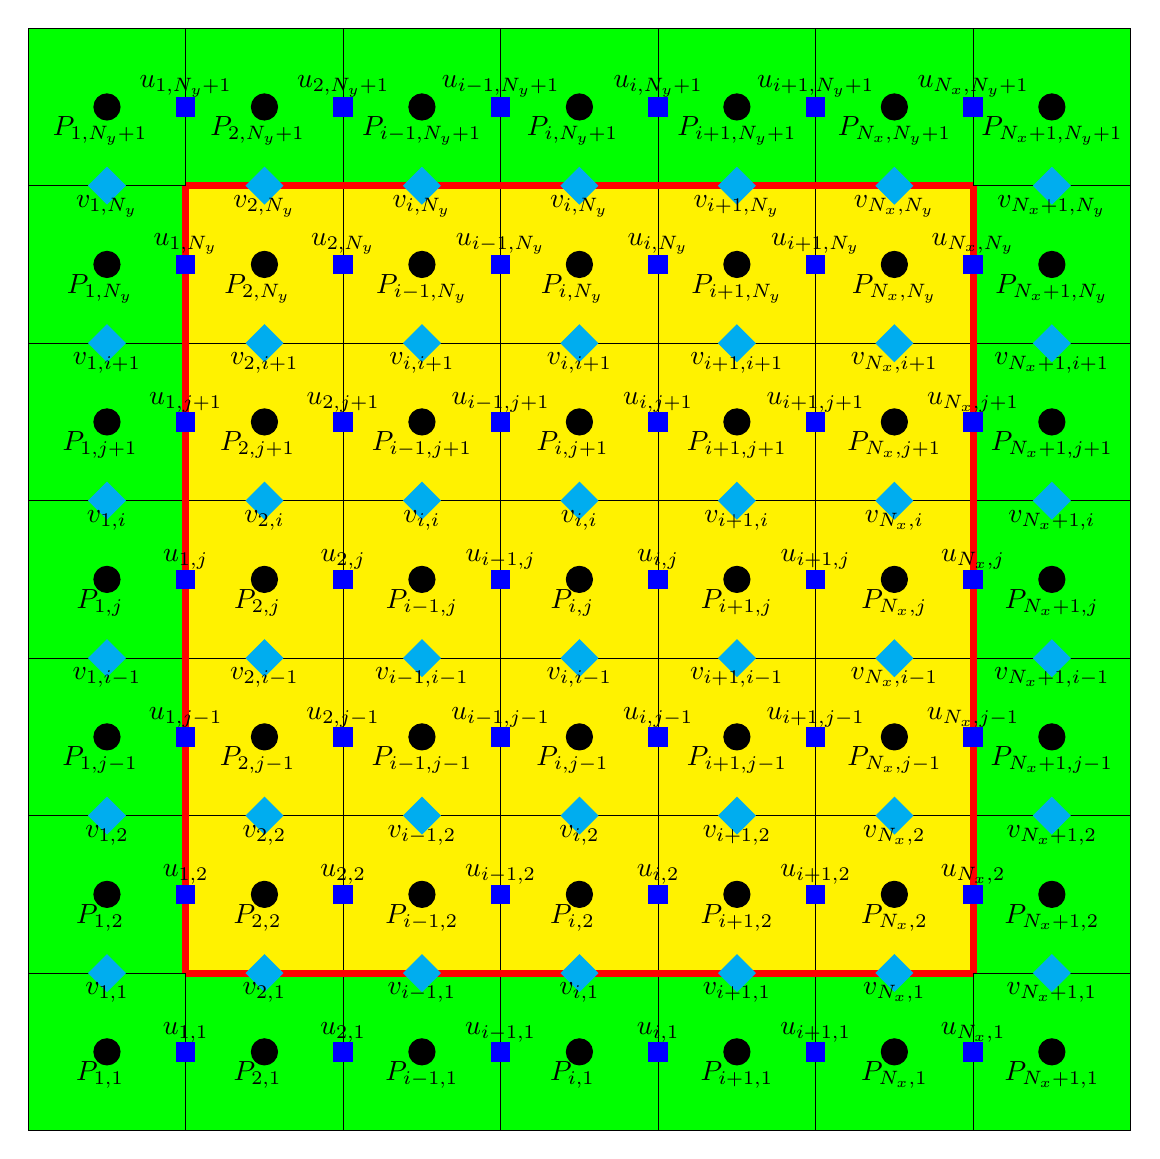
\begin{tikzpicture}
% Top grid
\draw [fill=green] (0,12) rectangle (2,14);
\draw [fill=green] (2,12) rectangle (4,14);
\draw [fill=green] (4,12) rectangle (6,14);
\draw [fill=green] (6,12) rectangle (8,14);
\draw [fill=green] (8,12) rectangle (10,14);
\draw [fill=green] (10,12) rectangle (12,14);
\draw [fill=green] (12,12) rectangle (14,14);
% Right Column
\draw [fill=green] (12,2) rectangle (14,4);
\draw [fill=green] (12,4) rectangle (14,6);
\draw [fill=green] (12,6) rectangle (14,8);
\draw [fill=green] (12,8) rectangle (14,10);
\draw [fill=green] (12,10) rectangle (14,12);
% Left Column
\draw [fill=green] (0,2) rectangle (2,4);
\draw [fill=green] (0,4) rectangle (2,6);
\draw [fill=green] (0,6) rectangle (2,8);
\draw [fill=green] (0,8) rectangle (2,10);
\draw [fill=green] (0,10) rectangle (2,12);
% Bottom grid
\draw [fill=green] (0,0) rectangle (2,2);
\draw [fill=green] (2,0) rectangle (4,2);
\draw [fill=green] (4,0) rectangle (6,2);
\draw [fill=green] (6,0) rectangle (8,2);
\draw [fill=green] (8,0) rectangle (10,2);
\draw [fill=green] (10,0) rectangle (12,2);
\draw [fill=green] (12,0) rectangle (14,2);
% Inner grid
\draw [fill=yellow] (2,2) rectangle (4,4);
\draw [fill=yellow] (4,2) rectangle (6,4);
\draw [fill=yellow] (6,2) rectangle (8,4);
\draw [fill=yellow] (8,2) rectangle (10,4);
\draw [fill=yellow] (10,2) rectangle (12,4);

\draw [fill=yellow] (2,4) rectangle (4,6);
\draw [fill=yellow] (4,4) rectangle (6,6);
\draw [fill=yellow] (6,4) rectangle (8,6);
\draw [fill=yellow] (8,4) rectangle (10,6);
\draw [fill=yellow] (10,4) rectangle (12,6);

\draw [fill=yellow] (2,6) rectangle (4,8);
\draw [fill=yellow] (4,6) rectangle (6,8);
\draw [fill=yellow] (6,6) rectangle (8,8);
\draw [fill=yellow] (8,6) rectangle (10,8);
\draw [fill=yellow] (10,6) rectangle (12,8);

\draw [fill=yellow] (2,8) rectangle (4,10);
\draw [fill=yellow] (4,8) rectangle (6,10);
\draw [fill=yellow] (6,8) rectangle (8,10);
\draw [fill=yellow] (8,8) rectangle (10,10);
\draw [fill=yellow] (10,8) rectangle (12,10);

\draw [fill=yellow] (2,10) rectangle (4,12);
\draw [fill=yellow] (4,10) rectangle (6,12);
\draw [fill=yellow] (6,10) rectangle (8,12);
\draw [fill=yellow] (8,10) rectangle (10,12);
\draw [fill=yellow] (10,10) rectangle (12,12);
% Red lines
\draw [red, line width=2.5] (2,2) -- (12,2);
\draw [red, line width=2.5] (2,2) -- (2,12);
\draw [red, line width=2.5] (12,2) -- (12,12);
\draw [red, line width=2.5] (2,12) -- (12,12);
% Points
\node at (1,1) [fill, circle, draw] {};
\node at (3,1) [fill, circle, draw] {};
\node at (5,1) [fill, circle, draw] {};
\node at (7,1) [fill, circle, draw] {};
\node at (9,1) [fill, circle, draw] {};
\node at (11,1) [fill, circle, draw] {};
\node at (13,1) [fill, circle, draw] {};

\node at (2,1) [draw,fill,rectangle,blue] {};
\node at (4,1) [draw,fill,rectangle,blue] {};
\node at (6,1) [draw,fill,rectangle,blue] {};
\node at (8,1) [draw,fill,rectangle,blue] {};
\node at (10,1) [draw,fill,rectangle,blue] {};
\node at (12,1) [draw,fill,rectangle,blue] {};

\node at (1,2) [draw, fill, diamond, cyan] {};
\node at (3,2) [draw, fill, diamond, cyan] {};
\node at (5,2) [draw, fill, diamond, cyan] {};
\node at (7,2) [draw, fill, diamond, cyan] {};
\node at (9,2) [draw, fill, diamond, cyan] {};
\node at (11,2) [draw, fill, diamond, cyan] {};
\node at (13,2) [draw, fill, diamond, cyan] {};

% 2nd row
\node at (1,3) [fill, circle, draw] {};
\node at (3,3) [fill, circle, draw] {};
\node at (5,3) [fill, circle, draw] {};
\node at (7,3) [fill, circle, draw] {};
\node at (9,3) [fill, circle, draw] {};
\node at (11,3) [fill, circle, draw] {};
\node at (13,3) [fill, circle, draw] {};

\node at (2,3) [draw,fill,rectangle,blue] {};
\node at (4,3) [draw,fill,rectangle,blue] {};
\node at (6,3) [draw,fill,rectangle,blue] {};
\node at (8,3) [draw,fill,rectangle,blue] {};
\node at (10,3) [draw,fill,rectangle,blue] {};
\node at (12,3) [draw,fill,rectangle,blue] {};

\node at (1,4) [draw, fill, diamond, cyan] {};
\node at (3,4) [draw, fill, diamond, cyan] {};
\node at (5,4) [draw, fill, diamond, cyan] {};
\node at (7,4) [draw, fill, diamond, cyan] {};
\node at (9,4) [draw, fill, diamond, cyan] {};
\node at (11,4) [draw, fill, diamond, cyan] {};
\node at (13,4) [draw, fill, diamond, cyan] {};

% 3rd row
\node at (1,5) [fill, circle, draw] {};
\node at (3,5) [fill, circle, draw] {};
\node at (5,5) [fill, circle, draw] {};
\node at (7,5) [fill, circle, draw] {};
\node at (9,5) [fill, circle, draw] {};
\node at (11,5) [fill, circle, draw] {};
\node at (13,5) [fill, circle, draw] {};

\node at (2,5) [draw,fill,rectangle,blue] {};
\node at (4,5) [draw,fill,rectangle,blue] {};
\node at (6,5) [draw,fill,rectangle,blue] {};
\node at (8,5) [draw,fill,rectangle,blue] {};
\node at (10,5) [draw,fill,rectangle,blue] {};
\node at (12,5) [draw,fill,rectangle,blue] {};

\node at (1,6) [draw, fill, diamond, cyan] {};
\node at (3,6) [draw, fill, diamond, cyan] {};
\node at (5,6) [draw, fill, diamond, cyan] {};
\node at (7,6) [draw, fill, diamond, cyan] {};
\node at (9,6) [draw, fill, diamond, cyan] {};
\node at (11,6) [draw, fill, diamond, cyan] {};
\node at (13,6) [draw, fill, diamond, cyan] {};

% 4th row
\node at (1,7) [fill, circle, draw] {};
\node at (3,7) [fill, circle, draw] {};
\node at (5,7) [fill, circle, draw] {};
\node at (7,7) [fill, circle, draw] {};
\node at (9,7) [fill, circle, draw] {};
\node at (11,7) [fill, circle, draw] {};
\node at (13,7) [fill, circle, draw] {};

\node at (2,7) [draw,fill,rectangle,blue] {};
\node at (4,7) [draw,fill,rectangle,blue] {};
\node at (6,7) [draw,fill,rectangle,blue] {};
\node at (8,7) [draw,fill,rectangle,blue] {};
\node at (10,7) [draw,fill,rectangle,blue] {};
\node at (12,7) [draw,fill,rectangle,blue] {};

\node at (1,8) [draw, fill, diamond, cyan] {};
\node at (3,8) [draw, fill, diamond, cyan] {};
\node at (5,8) [draw, fill, diamond, cyan] {};
\node at (7,8) [draw, fill, diamond, cyan] {};
\node at (9,8) [draw, fill, diamond, cyan] {};
\node at (11,8) [draw, fill, diamond, cyan] {};
\node at (13,8) [draw, fill, diamond, cyan] {};

% 5th row
\node at (1,9) [fill, circle, draw] {};
\node at (3,9) [fill, circle, draw] {};
\node at (5,9) [fill, circle, draw] {};
\node at (7,9) [fill, circle, draw] {};
\node at (9,9) [fill, circle, draw] {};
\node at (11,9) [fill, circle, draw] {};
\node at (13,9) [fill, circle, draw] {};

\node at (2,9) [draw,fill,rectangle,blue] {};
\node at (4,9) [draw,fill,rectangle,blue] {};
\node at (6,9) [draw,fill,rectangle,blue] {};
\node at (8,9) [draw,fill,rectangle,blue] {};
\node at (10,9) [draw,fill,rectangle,blue] {};
\node at (12,9) [draw,fill,rectangle,blue] {};

\node at (1,10) [draw, fill, diamond, cyan] {};
\node at (3,10) [draw, fill, diamond, cyan] {};
\node at (5,10) [draw, fill, diamond, cyan] {};
\node at (7,10) [draw, fill, diamond, cyan] {};
\node at (9,10) [draw, fill, diamond, cyan] {};
\node at (11,10) [draw, fill, diamond, cyan] {};
\node at (13,10) [draw, fill, diamond, cyan] {};


% 6th row
\node at (1,11) [fill, circle, draw] {};
\node at (3,11) [fill, circle, draw] {};
\node at (5,11) [fill, circle, draw] {};
\node at (7,11) [fill, circle, draw] {};
\node at (9,11) [fill, circle, draw] {};
\node at (11,11) [fill, circle, draw] {};
\node at (13,11) [fill, circle, draw] {};

\node at (2,11) [draw,fill,rectangle,blue] {};
\node at (4,11) [draw,fill,rectangle,blue] {};
\node at (6,11) [draw,fill,rectangle,blue] {};
\node at (8,11) [draw,fill,rectangle,blue] {};
\node at (10,11) [draw,fill,rectangle,blue] {};
\node at (12,11) [draw,fill,rectangle,blue] {};

\node at (1,12) [draw, fill, diamond, cyan] {};
\node at (3,12) [draw, fill, diamond, cyan] {};
\node at (5,12) [draw, fill, diamond, cyan] {};
\node at (7,12) [draw, fill, diamond, cyan] {};
\node at (9,12) [draw, fill, diamond, cyan] {};
\node at (11,12) [draw, fill, diamond, cyan] {};
\node at (13,12) [draw, fill, diamond, cyan] {};

% 7th row
\node at (1,13) [fill, circle, draw] {};
\node at (3,13) [fill, circle, draw] {};
\node at (5,13) [fill, circle, draw] {};
\node at (7,13) [fill, circle, draw] {};
\node at (9,13) [fill, circle, draw] {};
\node at (11,13) [fill, circle, draw] {};
\node at (13,13) [fill, circle, draw] {};

\node at (2,13) [draw,fill,rectangle,blue] {};
\node at (4,13) [draw,fill,rectangle,blue] {};
\node at (6,13) [draw,fill,rectangle,blue] {};
\node at (8,13) [draw,fill,rectangle,blue] {};
\node at (10,13) [draw,fill,rectangle,blue] {};
\node at (12,13) [draw,fill,rectangle,blue] {};

% Pressure labels
\node [below] at (1,1) {$P_{1,1}\phantom{1}$};
\node [below] at (3,1) {$P_{2,1}\phantom{1}$};
\node [below] at (5,1) {$P_{i-1,1}$};
\node [below] at (7,1) {$P_{i,1}\phantom{1}$};
\node [below] at (9,1) {$P_{i+1,1}$};
\node [below] at (11,1) {$P_{N_{x},1}$};
\node [below] at (13,1) {$P_{N_{x}+1,1}$};

\node [below] at (1,3) {$P_{1,2}\phantom{1}$};
\node [below] at (3,3) {$P_{2,2}\phantom{1}$};
\node [below] at (5,3) {$P_{i-1,2}$};
\node [below] at (7,3) {$P_{i,2}\phantom{1}$};
\node [below] at (9,3) {$P_{i+1,2}$};
\node [below] at (11,3) {$P_{N_{x},2}$};
\node [below] at (13,3) {$P_{N_{x}+1,2}$};

\node [below] at (1,5) {$P_{1,j-1}\phantom{1}$};
\node [below] at (3,5) {$P_{2,j-1}\phantom{1}$};
\node [below] at (5,5) {$P_{i-1,j-1}$};
\node [below] at (7,5) {$P_{i,j-1}\phantom{1}$};
\node [below] at (9,5) {$P_{i+1,j-1}$};
\node [below] at (11,5) {$P_{N_{x},j-1}$};
\node [below] at (13,5) {$P_{N_{x}+1,j-1}$};

\node [below] at (1,7) {$P_{1,j}\phantom{1}$};
\node [below] at (3,7) {$P_{2,j}\phantom{1}$};
\node [below] at (5,7) {$P_{i-1,j}$};
\node [below] at (7,7) {$P_{i,j}\phantom{1}$};
\node [below] at (9,7) {$P_{i+1,j}$};
\node [below] at (11,7) {$P_{N_{x},j}$};
\node [below] at (13,7) {$P_{N_{x}+1,j}$};

\node [below] at (1,9) {$P_{1,j+1}\phantom{1}$};
\node [below] at (3,9) {$P_{2,j+1}\phantom{1}$};
\node [below] at (5,9) {$P_{i-1,j+1}$};
\node [below] at (7,9) {$P_{i,j+1}\phantom{1}$};
\node [below] at (9,9) {$P_{i+1,j+1}$};
\node [below] at (11,9) {$P_{N_{x},j+1}$};
\node [below] at (13,9) {$P_{N_{x}+1,j+1}$};

\node [below] at (1,11) {$P_{1,N_{y}}\phantom{1}$};
\node [below] at (3,11) {$P_{2,N_{y}}\phantom{1}$};
\node [below] at (5,11) {$P_{i-1,N_{y}}$};
\node [below] at (7,11) {$P_{i,N_{y}}\phantom{1}$};
\node [below] at (9,11) {$P_{i+1,N_{y}}$};
\node [below] at (11,11) {$P_{N_{x},N_{y}}$};
\node [below] at (13,11) {$P_{N_{x}+1,N_{y}}$};

\node [below] at (1,13) {$P_{1,N_{y}+1}\phantom{1}$};
\node [below] at (3,13) {$P_{2,N_{y}+1}\phantom{1}$};
\node [below] at (5,13) {$P_{i-1,N_{y}+1}$};
\node [below] at (7,13) {$P_{i,N_{y}+1}\phantom{1}$};
\node [below] at (9,13) {$P_{i+1,N_{y}+1}$};
\node [below] at (11,13) {$P_{N_{x},N_{y}+1}$};
\node [below] at (13,13) {$P_{N_{x}+1,N_{y}+1}$};

% u terms
\node [above] at (2,1) {$u_{1,1}$};
\node [above] at (4,1) {$u_{2,1}$};
\node [above] at (6,1) {$u_{i-1,1}$};
\node [above] at (8,1) {$u_{i,1}$};
\node [above] at (10,1) {$u_{i+1,1}$};
\node [above] at (12,1) {$u_{N_{x},1}$};

\node [above] at (2,3) {$u_{1,2}$};
\node [above] at (4,3) {$u_{2,2}$};
\node [above] at (6,3) {$u_{i-1,2}$};
\node [above] at (8,3) {$u_{i,2}$};
\node [above] at (10,3) {$u_{i+1,2}$};
\node [above] at (12,3) {$u_{N_{x},2}$};


\node [above] at (2,5) {$u_{1,j-1}$};
\node [above] at (4,5) {$u_{2,j-1}$};
\node [above] at (6,5) {$u_{i-1,j-1}$};
\node [above] at (8,5) {$u_{i,j-1}$};
\node [above] at (10,5) {$u_{i+1,j-1}$};
\node [above] at (12,5) {$u_{N_{x},j-1}$};

\node [above] at (2,7) {$u_{1,j}$};
\node [above] at (4,7) {$u_{2,j}$};
\node [above] at (6,7) {$u_{i-1,j}$};
\node [above] at (8,7) {$u_{i,j}$};
\node [above] at (10,7) {$u_{i+1,j}$};
\node [above] at (12,7) {$u_{N_{x},j}$};

\node [above] at (2,9) {$u_{1,j+1}$};
\node [above] at (4,9) {$u_{2,j+1}$};
\node [above] at (6,9) {$u_{i-1,j+1}$};
\node [above] at (8,9) {$u_{i,j+1}$};
\node [above] at (10,9) {$u_{i+1,j+1}$};
\node [above] at (12,9) {$u_{N_{x},j+1}$};


\node [above] at (2,11) {$u_{1,N_{y}}$};
\node [above] at (4,11) {$u_{2,N_{y}}$};
\node [above] at (6,11) {$u_{i-1,N_{y}}$};
\node [above] at (8,11) {$u_{i,N_{y}}$};
\node [above] at (10,11) {$u_{i+1,N_{y}}$};
\node [above] at (12,11) {$u_{N_{x},N_{y}}$};

\node [above] at (2,13) {$u_{1,N_{y}+1}$};
\node [above] at (4,13) {$u_{2,N_{y}+1}$};
\node [above] at (6,13) {$u_{i-1,N_{y}+1}$};
\node [above] at (8,13) {$u_{i,N_{y}+1}$};
\node [above] at (10,13) {$u_{i+1,N_{y}+1}$};
\node [above] at (12,13) {$u_{N_{x},N_{y}+1}$};

% v terms
\node [below] at (1,2) {$v_{1,1}$};
\node [below] at (3,2) {$v_{2,1}$};
\node [below] at (5,2) {$v_{i-1,1}$};
\node [below] at (7,2) {$v_{i,1}$};
\node [below] at (9,2) {$v_{i+1,1}$};
\node [below] at (11,2) {$v_{N_{x},1}$};
\node [below] at (13,2) {$v_{N_{x}+1,1}$};


\node [below] at (1,4) {$v_{1,2}$};
\node [below] at (3,4) {$v_{2,2}$};
\node [below] at (5,4) {$v_{i-1,2}$};
\node [below] at (7,4) {$v_{i,2}$};
\node [below] at (9,4) {$v_{i+1,2}$};
\node [below] at (11,4) {$v_{N_{x},2}$};
\node [below] at (13,4) {$v_{N_{x}+1,2}$};


\node [below] at (1,6) {$v_{1,i-1}$};
\node [below] at (3,6) {$v_{2,i-1}$};
\node [below] at (5,6) {$v_{i-1,i-1}$};
\node [below] at (7,6) {$v_{i,i-1}$};
\node [below] at (9,6) {$v_{i+1,i-1}$};
\node [below] at (11,6) {$v_{N_{x},i-1}$};
\node [below] at (13,6) {$v_{N_{x}+1,i-1}$};


\node [below] at (1,8) {$v_{1,i}$};
\node [below] at (3,8) {$v_{2,i}$};
\node [below] at (5,8) {$v_{i,i}$};
\node [below] at (7,8) {$v_{i,i}$};
\node [below] at (9,8) {$v_{i+1,i}$};
\node [below] at (11,8) {$v_{N_{x},i}$};
\node [below] at (13,8) {$v_{N_{x}+1,i}$};


\node [below] at (1,10) {$v_{1,i+1}$};
\node [below] at (3,10) {$v_{2,i+1}$};
\node [below] at (5,10) {$v_{i,i+1}$};
\node [below] at (7,10) {$v_{i,i+1}$};
\node [below] at (9,10) {$v_{i+1,i+1}$};
\node [below] at (11,10) {$v_{N_{x},i+1}$};
\node [below] at (13,10) {$v_{N_{x}+1,i+1}$};

\node [below] at (1,12) {$v_{1,N_{y}}$};
\node [below] at (3,12) {$v_{2,N_{y}}$};
\node [below] at (5,12) {$v_{i,N_{y}}$};
\node [below] at (7,12) {$v_{i,N_{y}}$};
\node [below] at (9,12) {$v_{i+1,N_{y}}$};
\node [below] at (11,12) {$v_{N_{x},N_{y}}$};
\node [below] at (13,12) {$v_{N_{x}+1,N_{y}}$};
\end{tikzpicture}
\caption{Entire staggered grid where the red line defines the standard boundary, the yellow boxes define the normal nodes and the green nodes define the ``ghost'' boundaries. The black circles represent the nodes for $P$, blue squares for $u$, and the cyan diamonds for $v$.}
\label{fig:stagg_grid}
\end{figure}

{\bf \large Boundary Conditions}

\begin{enumerate}
\item The ``ghost'' pressure terms are initialized to zero, as there shouldn't be any pressure outside of the original domain boundary. The edges of the pressure control volumes (Figure~\ref{fig:stagg_1}) coincide with the original domain of the system. Therefore, the {\em normal} velocities are specified directly at the walls.
\item The tangential velocities (velocities in the ``ghost boundaries'') is given by $U_{wall}$ to satisfy the no-slip condition. We can interpolate this linearly with the velocity inside the domain, also known as the reflection technique, which gives us:
\begin{align}
\frac{u_{i,2} + u_{i,1}}{2} &= U_{wall}\\
\intertext{where we can solve for the ``ghost'' velocity as}
u_{i,1} &= 2U_{wall} - u_{i,2}
\end{align}
\end{enumerate}

{\bf \large Solving the Pressure Equation}

We can get the equation for the pressure by taking Equation~\ref{eq:vel_corr} and plugging it into Equation~\ref{eq:vel_constraint} after discritizing gives us:

\begin{align}
P_{i+1,j} + P_{i-1,j} + P_{i,j+1} + P_{i,j-1} - 4P_{i,j} &= \frac{h}{\Delta t} \left( u_{i+\frac{1}{2},j}^{t} - u^{t}_{i-\frac{1}{2},j} + v^{t}_{i,j+\frac{1}{2}} - v^{t}_{i,j-\frac{1}{2}}\right)
\end{align}
where, solving for $P_{i,j}$ gives
\begin{align}
P_{i,j} &= \xi_{i,j}\left[ \left(P_{i+1,j} + P_{i-1,j} + P_{i,j+1} + P_{i,j-1}\right) - \frac{h}{\Delta t} \left( u_{i,j}^{t} - u_{i-1,j}^{t} + v_{i,j}^{t}-v_{i,j-1}^{t}\right)\right]
\end{align}

where $\xi_{i,j}$ is dependent upon the current node being solved. For example, as referring to Figure~\ref{fig:stagg_grid}, if a node is at a single wall boundary, one of the pressures in the ``ghost domain'' is zero, so $\xi_{i,j}$ would only be $\frac{1}{3}$ since only 3 pressure terms contribute to the system. At a corner, $\xi_{i,j} = \frac{1}{2}$ since two of the pressure terms will be zero, and for every other index $\xi_{i,j} = \frac{1}{4}$ as per the original equation.

{\bf \large Vorticity}

The voriticy of the system can be calculated as

\begin{align}
\omega &= \frac{\text{d}v}{\text{d}x} - \frac{\text{d}u}{\text{d}y}
\end{align}

{\bf \large Results} 

As the case for $R_{e} = 100$ was performed in the last assignment, it was easy to test to see if the code performed correctly by running it for this case and comparing it to the results of the last assignment. This turned out to produce exaclty the same result as the last assignment, so we could say that the result of this code was taken to be working. It also seemed to agree with the physics of it as well, as one would expect that it would rotate clockwise around the cavity. This is seen in Figure~\ref{fig:vorticity_streamfunction_re100}.

The results can be analyzed by looking at the pressure of the system as well. As we know from the basic principles of systems, a flow should tend towards and speed up towards low pressure systems and be pushed away from high pressure areas. With the top lid flowing to the right of the system, we expect a high pressure to appear on the top right corner and a low pressure on the left. This would cause the rotation to occur. This is exactly what is represented in Figure~\ref{fig:pressure_re100}.

For each of these examples, $U_{wall}=10$ for the top, and $U_{wall}=0$ for the other walls. For convergence of the system, convergence for various Reynolds numbers was determined by looking at the Poisson Equation for Pressure. In looking at the Numerical Convergence of the system, we came to the result that the following value for $\Delta t$ had to be used for convergence to happen, which was

\begin{align}
\frac{\nu \Delta t}{h^{2}} \leq \frac{1}{4}
\intertext{though to guarentee convergence, we made it such that}
\Delta t = \frac{h^{2}}{40\nu}
\end{align}

which took care of any unforseen irregularities that may be seen for various Reynolds Flows.

\begin{figure}[H]
\centering
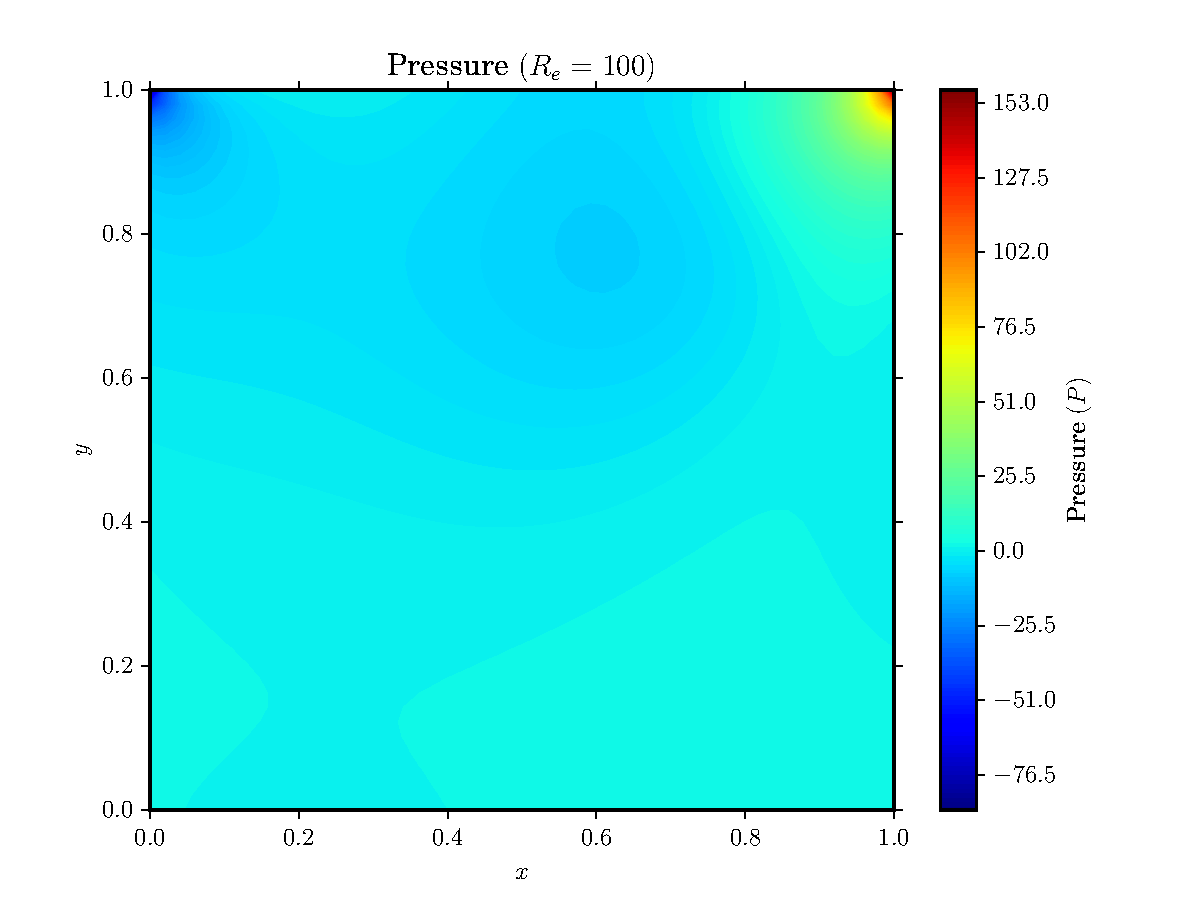
\includegraphics[width=.75\textwidth]{figs/pressure_100.pdf}
\caption{Pressure for $R_{e}=100$}
\label{fig:pressure_re100}
\end{figure}

\begin{figure}[H]
\centering
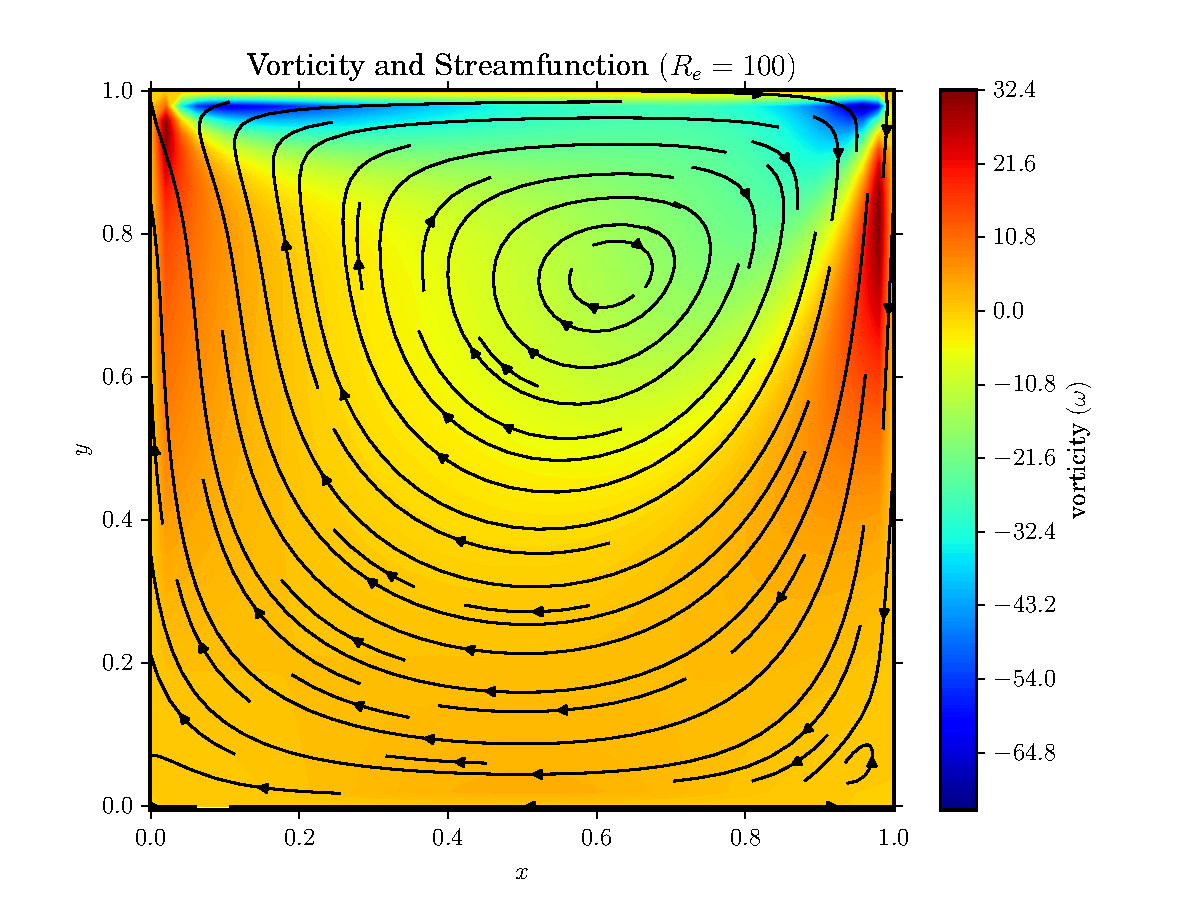
\includegraphics[width=.75\textwidth]{figs/vorticity_streamfunction_100.pdf}
\caption{Vorticity and Streamfunction for $R_{e}=100$}
\label{fig:vorticity_streamfunction_re100}
\end{figure}

\begin{figure}[H]
\centering
\begin{minipage}{.45\textwidth}
\centering
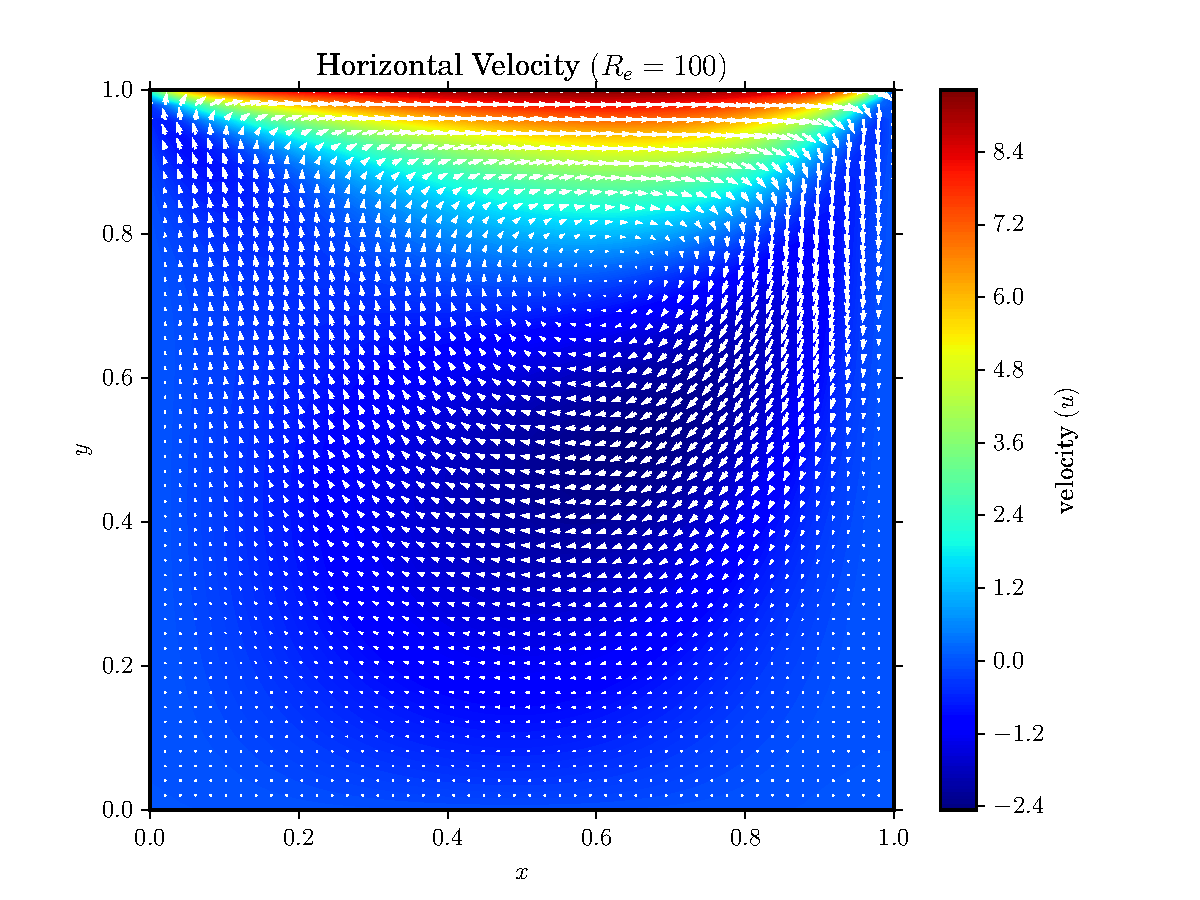
\includegraphics[width=\textwidth]{figs/x-velocity_100.pdf}
\captionof{figure}{$x$-velocity for $R_{e}=100$}
\label{fig:x_vel_re100}
\end{minipage}
\begin{minipage}{.45\textwidth}
\centering
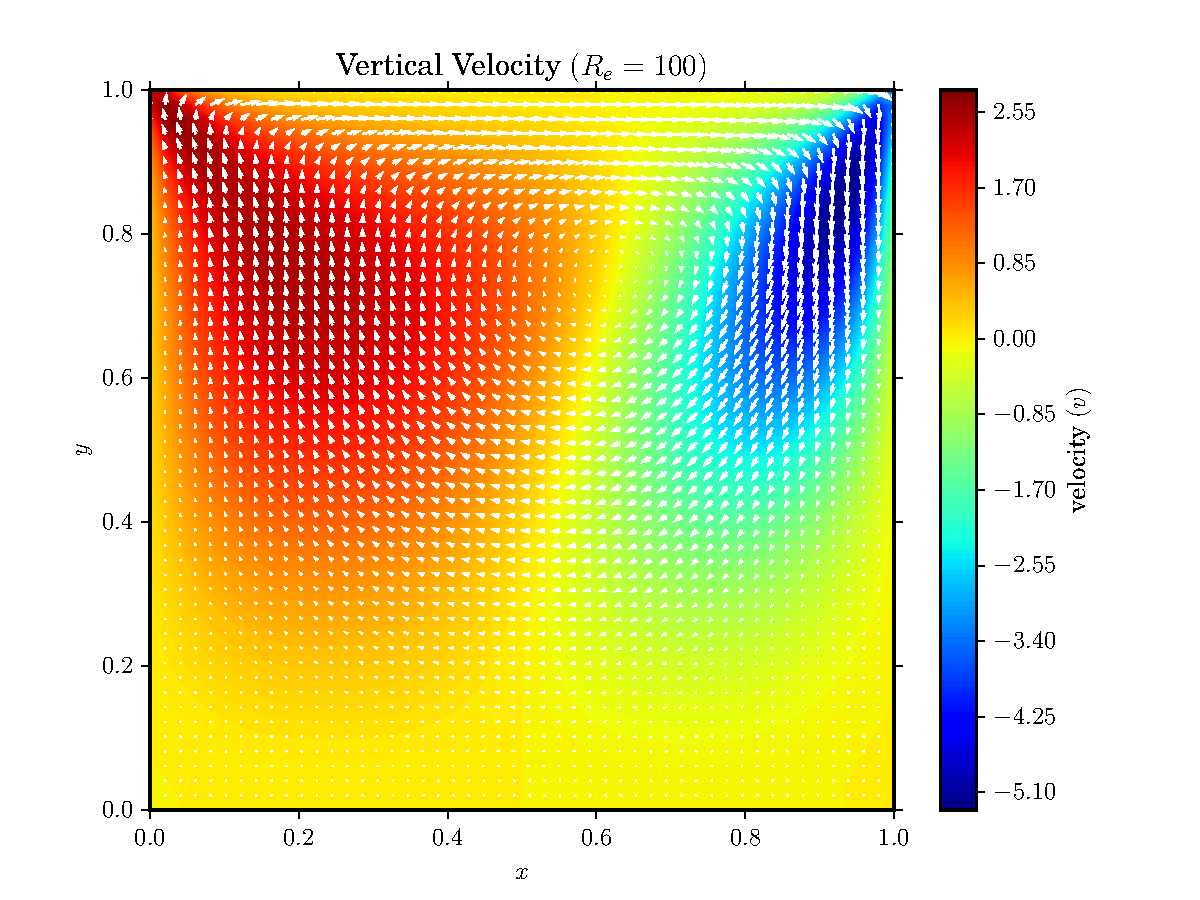
\includegraphics[width=\textwidth]{figs/y-velocity_100.pdf}
\captionof{figure}{$y$-velocity for $R_{e}=100$}
\label{fig:y_vel_re100}
\end{minipage}
\end{figure}


As we have tested for the main case which we know works $(R_{e}=100)$, we can now test systems with other Reynolds numbers. For the low Reynolds number case, we opted to test it for with $R_{e}=10$. The results for the vorticity and streamfunction can be seen in Figure~\ref{fig:vorticity_streamfunction_re10}, which shows the results that we expect. As the Reynolds number decreases, we expect the fluid to keep less structure as it is less viscous than fluids with higher Reynolds numbers. The case where $R_{e}=1$ was also tested, though it produced the same result as $R_{e}=10$. 

\begin{figure}[H]
\centering
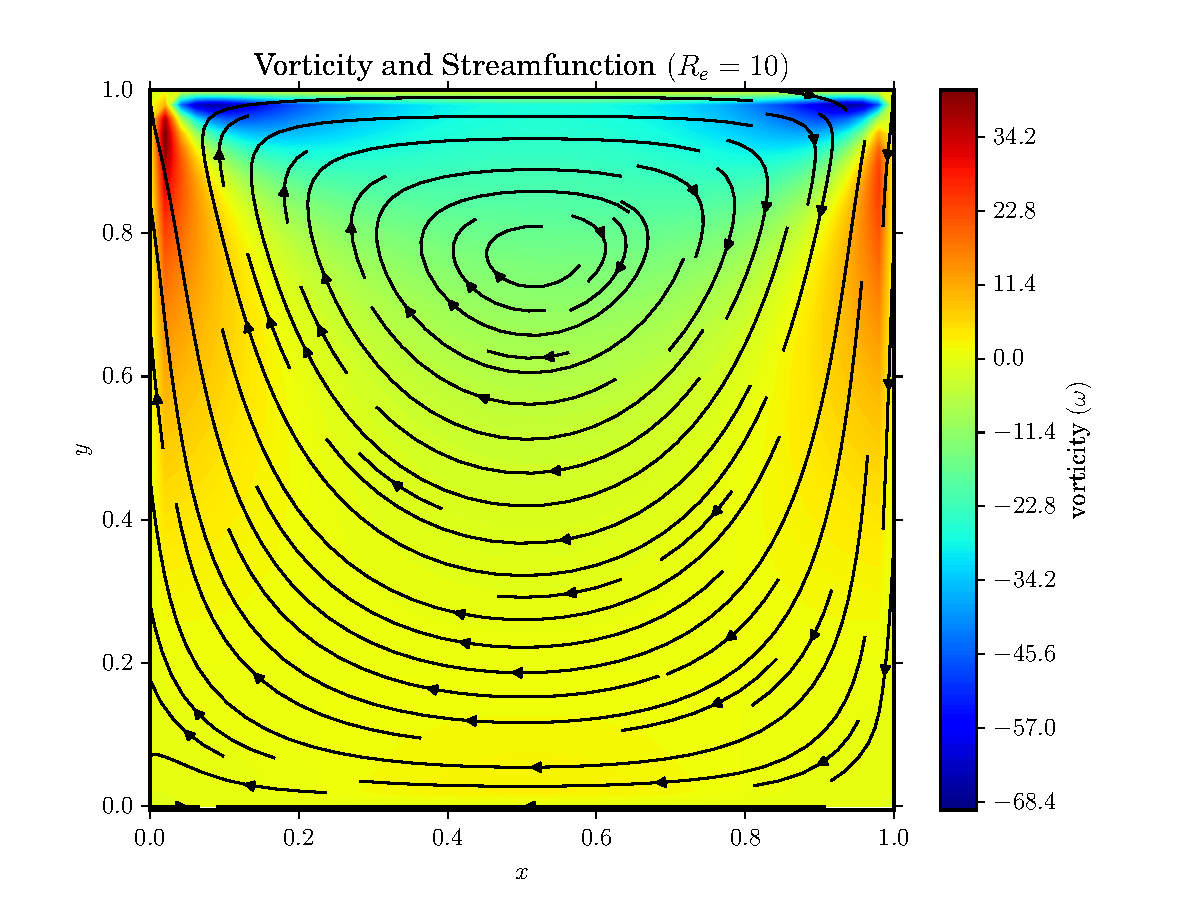
\includegraphics[width=.75\textwidth]{figs/vorticity_streamfunction_10.pdf}
\caption{Vorticity and Streamfunction for $R_{e}=10$}
\label{fig:vorticity_streamfunction_re10}
\end{figure}

\begin{figure}[H]
\centering
\begin{minipage}{.45\textwidth}
\centering
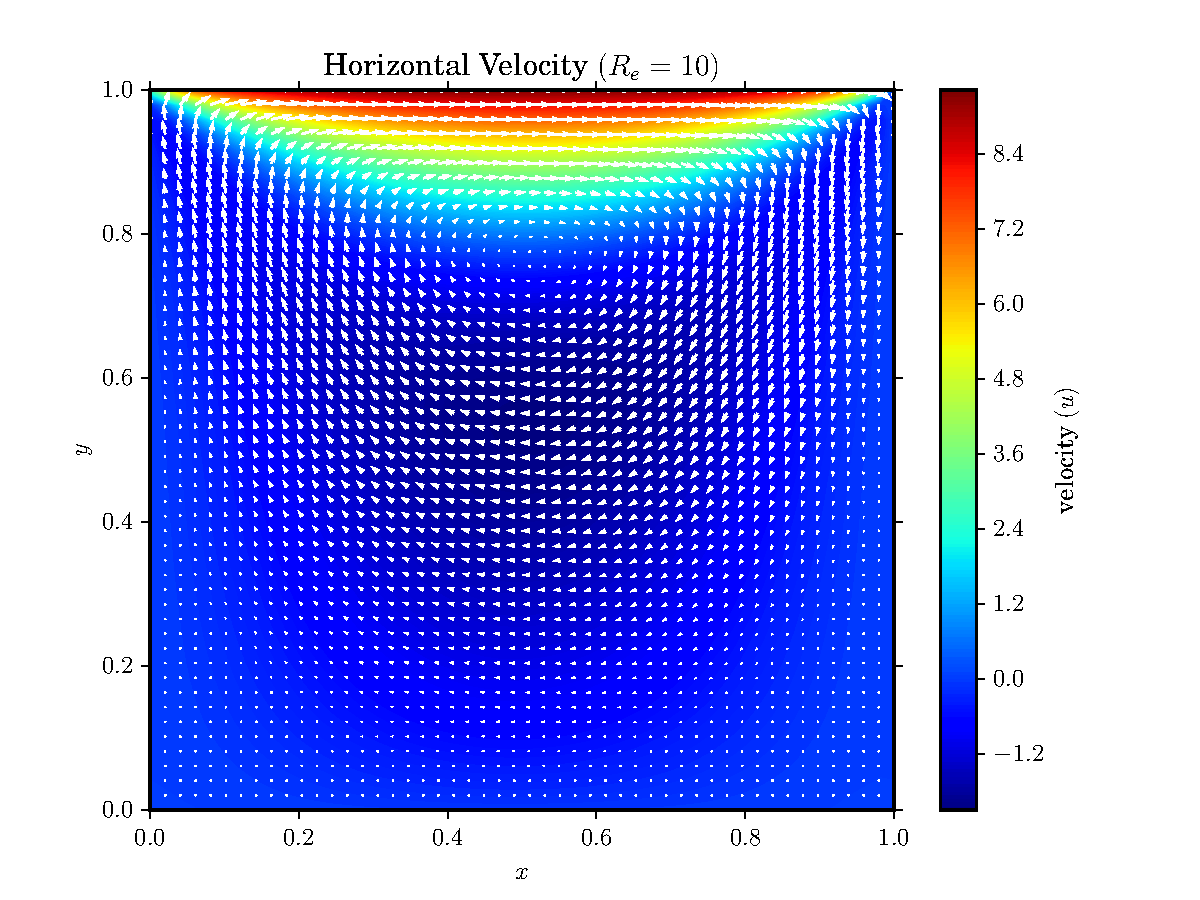
\includegraphics[width=\textwidth]{figs/x-velocity_10.pdf}
\captionof{figure}{$x$-velocity for $R_{e}=10$}
\label{fig:x_vel_re10}
\end{minipage}
\begin{minipage}{.45\textwidth}
\centering
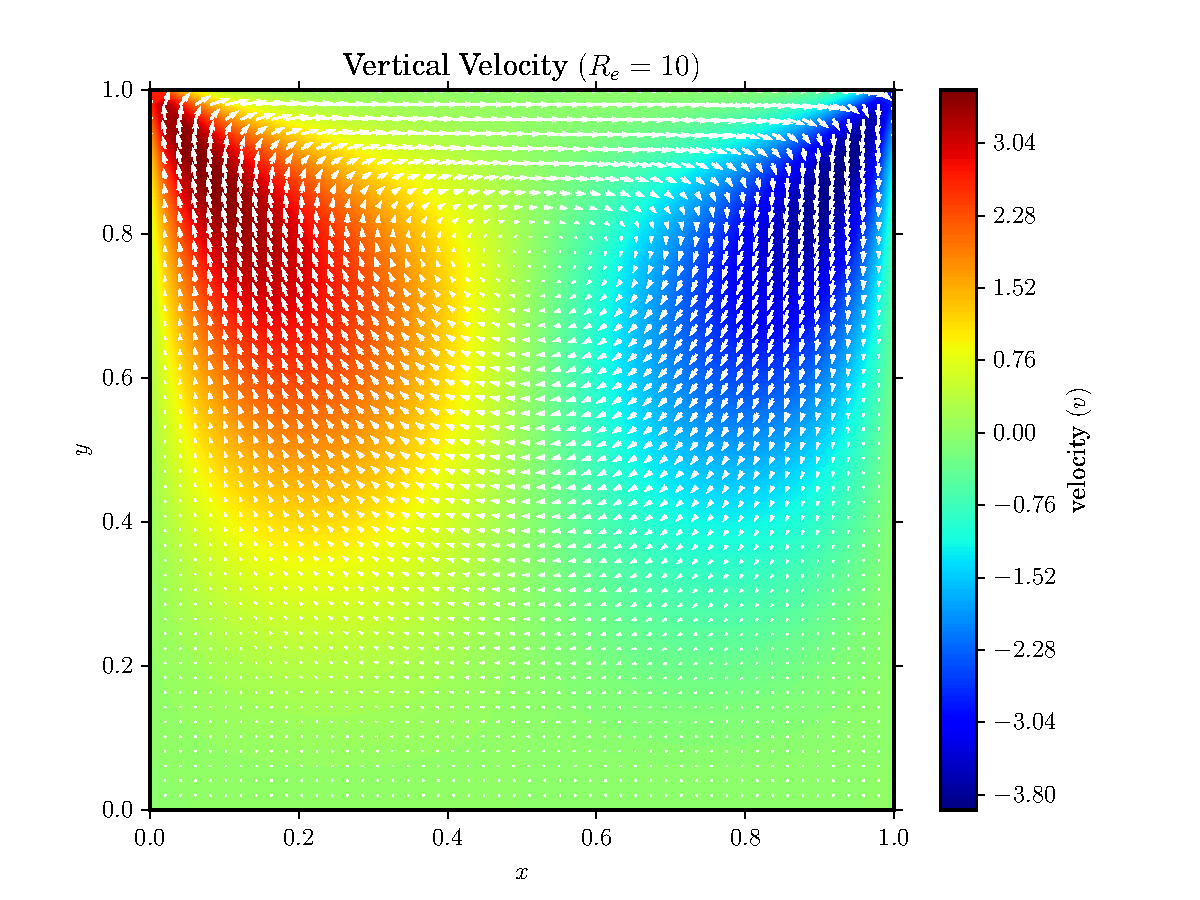
\includegraphics[width=\textwidth]{figs/y-velocity_10.pdf}
\captionof{figure}{$y$-velocity for $R_{e}=10$}
\label{fig:y_vel_re10}
\end{minipage}
\end{figure}


Finally, we performed the results for a high Reynolds number case where $R_{e}=1000$. As can be seen in Figure~\ref{fig:vorticity_streamfunction_re1000}, this fluid keeps its structure a lot better than the others. This is due to it being more viscous than the other examples. 

\begin{figure}[H]
\centering
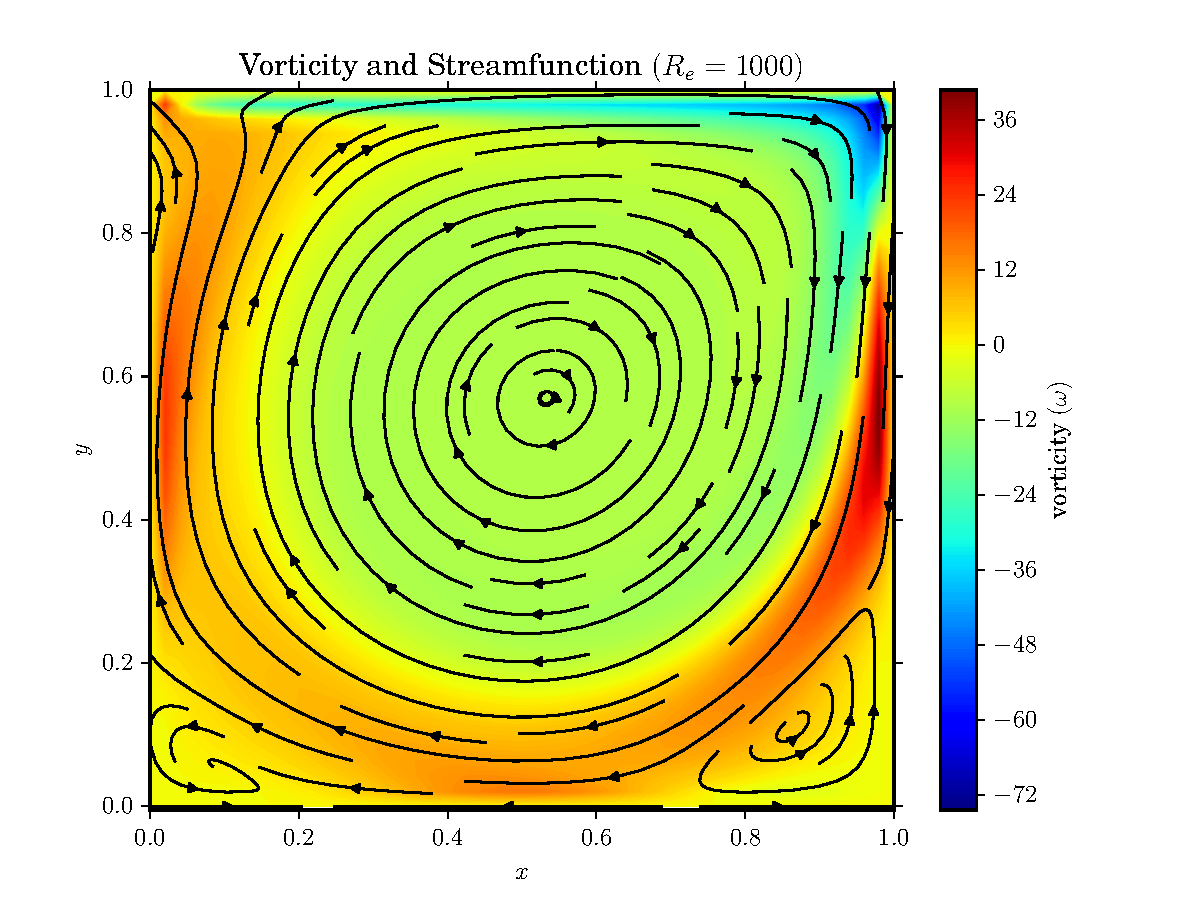
\includegraphics[width=.75\textwidth]{figs/vorticity_streamfunction_1000.pdf}
\caption{Vorticity and Streamfunction for $R_{e}=1000$}
\label{fig:vorticity_streamfunction_re1000}
\end{figure}

\begin{figure}[H]
\centering
\begin{minipage}{.45\textwidth}
\centering
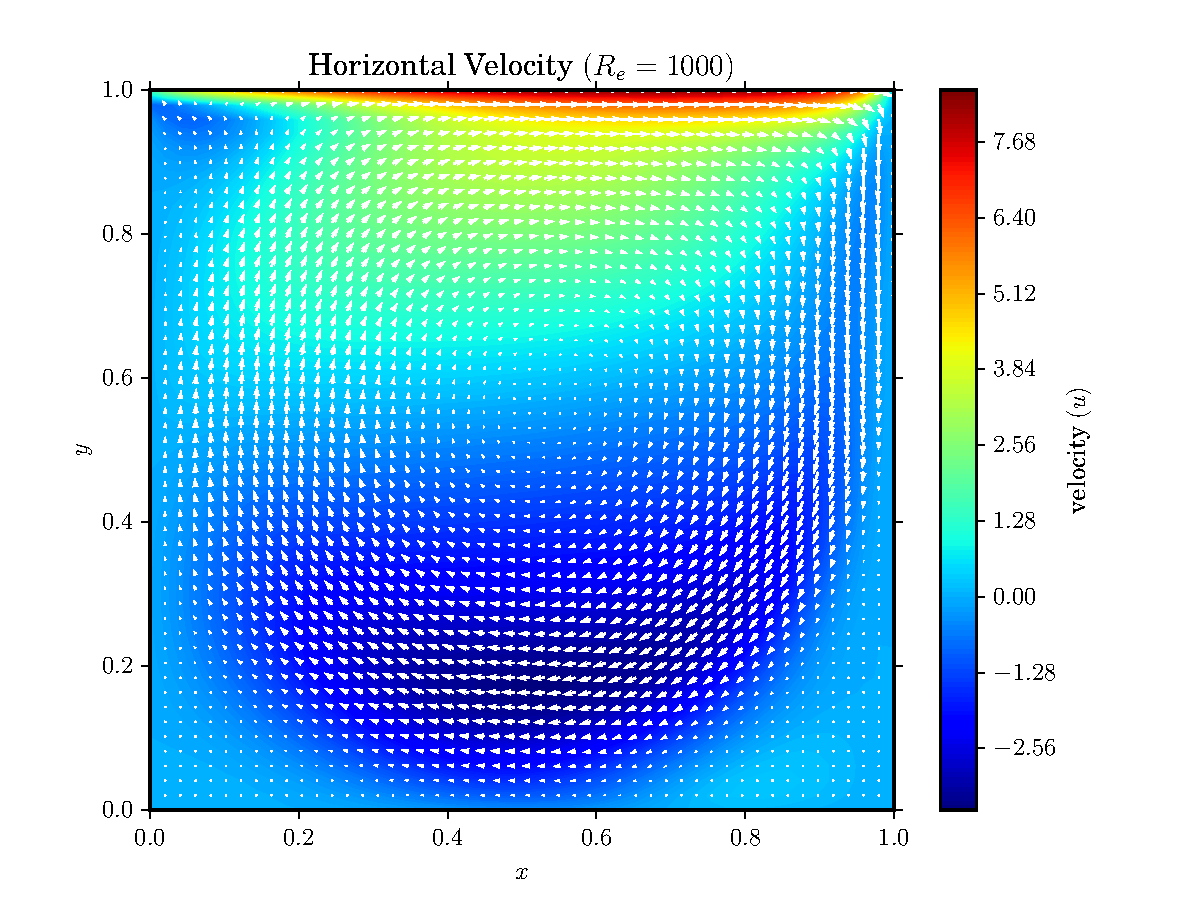
\includegraphics[width=\textwidth]{figs/x-velocity_1000.pdf}
\captionof{figure}{$x$-velocity for $R_{e}=1000$}
\label{fig:x_vel_re1000}
\end{minipage}
\begin{minipage}{.45\textwidth}
\centering
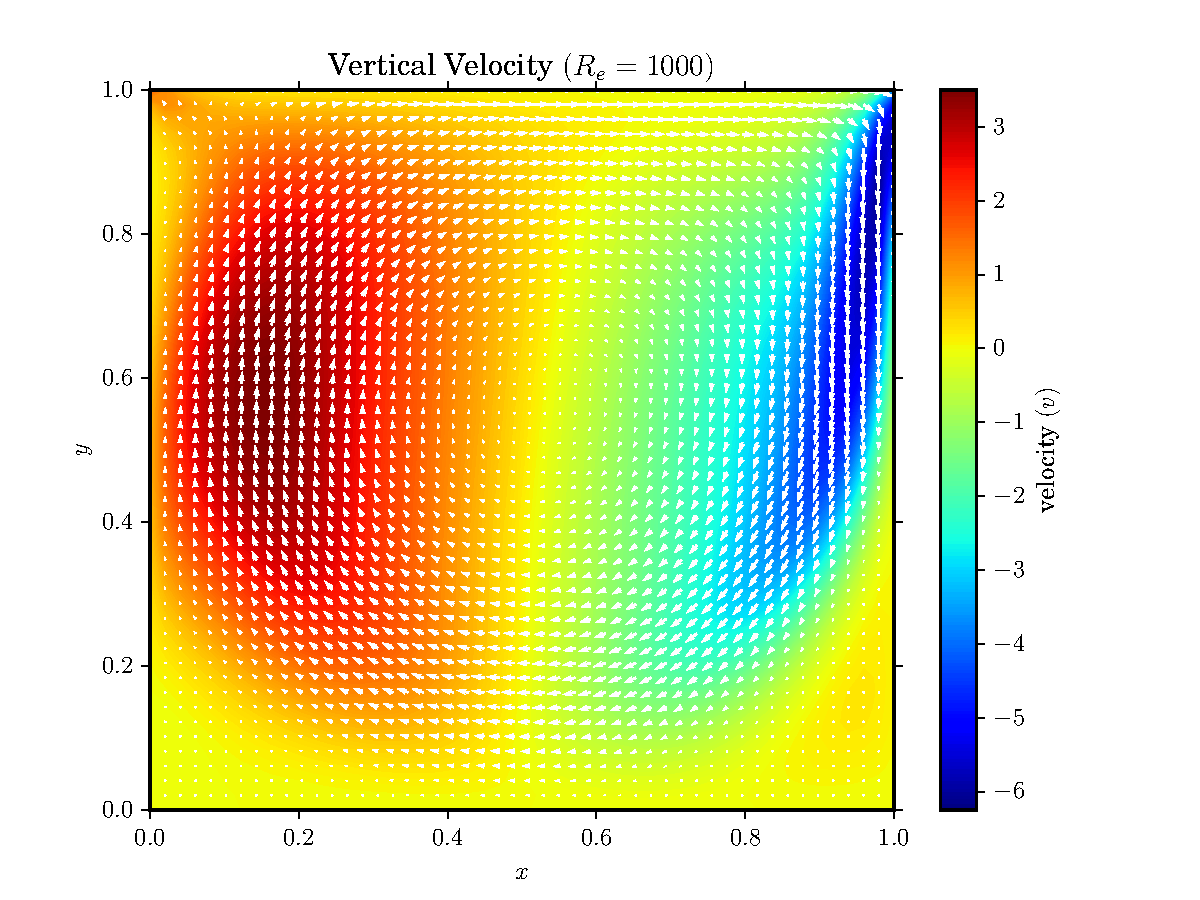
\includegraphics[width=\textwidth]{figs/y-velocity_1000.pdf}
\captionof{figure}{$y$-velocity for $R_{e}=1000$}
\label{fig:y_vel_re1000}
\end{minipage}
\end{figure}

\end{solution}

\end{questions}

%\begin{thebibliography}{99}
%\bibitem{box}John C. Tannehill, {\em et. al}, {\em Computational Fluid Mechanics and Heat Transfer}
%\end{thebibliography}

\end{document}

%%% Local Variables:
%%% mode: latex
%%% TeX-master: t
%%% End:
